\documentclass[journal]{IEEEtran}
\usepackage{cite}
\usepackage{amsmath,amssymb,amsfonts}
\usepackage{algorithmic}
\usepackage{graphicx}
\usepackage{textcomp}
\usepackage{xcolor}
\usepackage{booktabs}
\usepackage{url}

\graphicspath{{figures/}}

\newcommand{\FO}{\mathrm{FO}}

\begin{document}

\title{Hybrid Ant-Colony Metaheuristics for QoS-Aware Traffic-Engineering Optimization in Software-Defined Networks: Formulation, Simulation, and Testbed Validation}

\author{Jo\~{a}o~Paulo~Versiani~Ladeia~and~Nilton~Alves~Maia%
\thanks{J. P. Versiani Ladeia and N. A. Maia are with the Graduate Program in Computational Modeling and Systems (PPGMCS), Universidade Estadual de Montes Claros (Unimontes), Montes Claros -- MG, 39401-089, Brazil (e-mail: jpversiani@gmail.com, nilton.maia@unimontes.br).}}

\markboth{IEEE Transactions on Network and Service Management}{Versiani Ladeia \& Maia: Hybrid Metaheuristics for QoS-Aware SDN Traffic Engineering}

\maketitle

\begin{abstract}
The explosive proliferation of multimedia applications, cloud services, and bandwidth-intensive Internet workloads imposes stringent Quality of Service (QoS) guarantees on modern network infrastructures. Traditional routing protocols relying on shortest-path metrics (such as OSPF and IS-IS) frequently congest critical core links while leaving parallel paths underutilized, provoking severe bufferbloat, packet loss, and jitter. Software-Defined Networking (SDN) overcomes these architectural limitations by centralizing control plane intelligence and enabling dynamic, flow-level traffic engineering (TE). In this paper, we formulate the multi-flow QoS routing problem in an SDN as a combinatorial optimization model that simultaneously accounts for end-to-end latency bounds, link capacity constraints, and differentiated application priorities. To solve this NP-hard problem efficiently, we design a two-stage hybrid metaheuristic framework: first, an Ant Colony Optimization (ACO) algorithm inspired by AntNet explores the topology to construct a diverse pool of loop-free candidate paths; second, a Genetic Algorithm (ACO$+$GA) or Differential Evolution (ACO$+$DE) performs global combinatorial selection to identify the optimal route assignment. We conduct an extensive dual-track evaluation: an algorithmic benchmark against Dijkstra and Constrained Shortest Path First (CSPF) baselines under varying traffic loads, combined with empirical validation on a full-scale OpenFlow emulation testbed consisting of 52 switches orchestrated by a Floodlight controller and evaluated with the Distributed Internet Traffic Generator (D-ITG). In our empirical testbed experiments with 17 concurrent heterogeneous application flows, the optimized network achieves a 34.45\% higher average throughput, a 51.19$\times$ lower end-to-end delay (mitigating severe bufferbloat from 10.79~s down to 0.21~s), a 7.49$\times$ lower jitter, and a 510.4$\times$ reduction in packet loss compared to the shortest-path baseline. Furthermore, load stress testing confirms that the hybrid optimizer preserves link utilization below 100\% under heavy traffic where greedy and shortest-path baselines suffer acute congestion.
\end{abstract}

\begin{IEEEkeywords}
Software-Defined Networking (SDN), Traffic Engineering (TE), Quality of Service (QoS), Ant Colony Optimization (ACO), Genetic Algorithm (GA), Differential Evolution (DE), Bufferbloat, Mininet, OpenFlow.
\end{IEEEkeywords}

\section{Introduction}
\IEEEPARstart{O}{ver} the past two decades, global communication networks have experienced an unprecedented transformation in traffic volume, user density, and service heterogeneity~\cite{kreutz2015software}. Driven by high-definition video streaming, real-time conferencing, mobile cloud computing, and Internet of Things (IoT) deployments, global Internet traffic continues to expand at exponential rates. Network operators face the relentless challenge of satisfying diverse Quality of Service (QoS) constraints---such as strict upper bounds on end-to-end latency, bounded delay variation (jitter), and negligible packet loss---while containing capital expenditures (CapEx) and operational expenditures (OpEx)~\cite{wang2008qos}. Under these circumstances, continually upgrading physical link capacities is economically unfeasible and technically insufficient. 

Traffic Engineering (TE) addresses this fundamental challenge by intelligently routing, steering, and dimensioning network traffic across existing resources~\cite{awduche2002overview, fortz2002traffic}. However, implementing sophisticated TE mechanisms in legacy IP architectures has historically been hindered by the distributed and closed nature of traditional routers. Conventional interior gateway protocols, such as Open Shortest Path First (OSPF) and Intermediate System to Intermediate System (IS-IS), calculate routes independently at each node using localized shortest-path algorithms (e.g., Dijkstra's algorithm~\cite{dijkstra1959note}). Because shortest-path routing directs all flows along hop-minimal or distance-minimal paths, shared bottleneck links frequently become severely congested while alternative paths remain idle. This asymmetry results in packet buffering, severe bufferbloat~\cite{gettys2011bufferbloat}, and substantial degradation of real-time multimedia flows.

Software-Defined Networking (SDN) breaks this paradigm by decoupling the control plane from the underlying data-forwarding hardware~\cite{mckeown2008openflow, nunes2014survey}. By centralizing network state in a programmable software controller, SDN provides global visibility of topology, traffic matrices, and link utilization. Through standard southbound protocols like OpenFlow, the controller can push fine-grained forwarding rules directly into switch flow tables. This native programmability transforms SDN into an ideal platform for implementing global, QoS-aware traffic engineering~\cite{kim2013improving, jain2013b4, hong2013achieving, agarwal2013traffic}.

Despite the architectural advantages of SDN, computing optimal forwarding paths for multiple concurrent flows under QoS constraints remains an NP-hard multi-constrained combinatorial problem~\cite{korkmaz2001multiconstrained, lin2022survey}. Exact integer linear programming (ILP) solvers become computationally intractable as the network size and flow count scale. Consequently, metaheuristics and evolutionary computing provide an attractive trade-off between computational tractability and solution quality~\cite{dorigo2004ant, goldberg1989genetic, storn1997differential, alsadi2021qos}.

In this paper, we propose a comprehensive, two-stage hybrid metaheuristic architecture for QoS-aware traffic engineering in SDNs. Our framework decouples path exploration from global combinatorial route selection:
\begin{enumerate}
    \item \textbf{Stage 1 (Path Pool Exploration):} An Ant Colony Optimization (ACO) algorithm, based on the stigmergetic principles of AntNet~\cite{dicaro1998antnet}, explores the network topology to construct a diverse set of loop-free candidate paths for each active application.
    \item \textbf{Stage 2 (Global Combinatorial Selection):} Evolutionary algorithms---specifically a Genetic Algorithm (ACO$+$GA) and Differential Evolution (ACO$+$DE)---search the multi-application solution space to select an optimal vector of routes that maximizes a multi-criteria QoS objective function.
\end{enumerate}

To establish the practical validity of our approach, we perform a dual-track experimental evaluation: an algorithmic study comparing the proposed hybrids against Dijkstra and Constrained Shortest Path First (CSPF) baselines under varying traffic loads, and an empirical evaluation deployed on a realistic 52-node OpenFlow emulation testbed orchestrated with Mininet~\cite{lantz2010network}, Floodlight, and the Distributed Internet Traffic Generator (D-ITG)~\cite{botta2012itg}.

The remainder of this paper is structured as follows. Section~\ref{sec:related} surveys related work in SDN traffic engineering and QoS routing. Section~\ref{sec:model} establishes the mathematical model and objective function. Section~\ref{sec:methodology} describes the hybrid metaheuristic algorithms. Section~\ref{sec:setup} details the experimental setup and evaluation methodology. Section~\ref{sec:results} presents the algorithmic and empirical testbed results alongside a discussion of the bufferbloat phenomenon. Finally, Section~\ref{sec:conclusion} concludes the paper and outlines future directions.

\begin{figure}[!t]
\centering
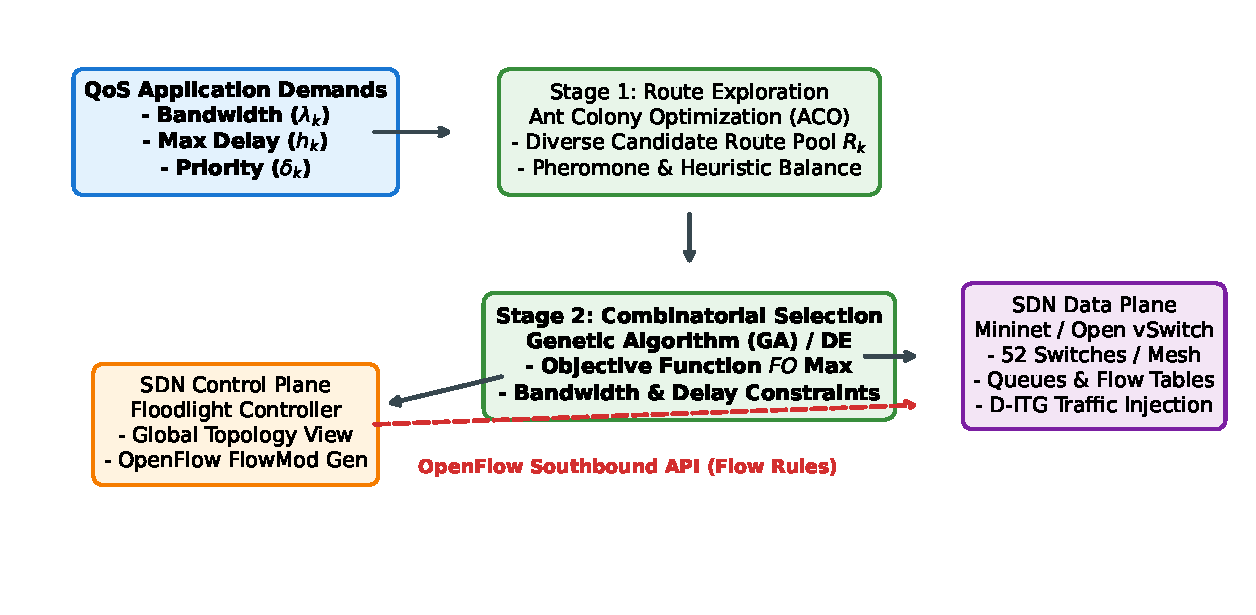
\includegraphics[width=\columnwidth]{fig1_architecture.pdf}
\caption{End-to-end architecture of the proposed QoS-aware SDN traffic engineering framework, illustrating the two-stage hybrid optimization engine and OpenFlow testbed deployment.}
\label{fig:arch}
\end{figure}

%---------------------------------------------------------------------
\section{Related Work}
\label{sec:related}
Traffic engineering has been a core research topic since the inception of connection-oriented MPLS and constraint-based routing~\cite{awduche2002overview}. In traditional IP networks, TE is typically achieved by optimizing OSPF link weights~\cite{fortz2002traffic}. However, weight optimization is inherently indirect, coarse-grained, and slow to adapt to dynamic traffic shifts.

With the advent of SDN, centralized traffic management gained widespread industry adoption. Google deployed B4~\cite{jain2013b4}, a private software-defined WAN connecting global data centers, achieving near 100\% link utilization through centralized bandwidth allocation and multi-path packet splitting. Microsoft implemented SWAN~\cite{hong2013achieving}, which coordinates inter-data-center traffic using centralized rate limiting and path computation. While B4 and SWAN target inter-datacenter WANs with elastic bulk transfers, enterprise and campus networks demand strict per-flow QoS guarantees for real-time interactive voice and video~\cite{kumar2021sdn, badotra2020qos}.

Metaheuristic approaches have emerged as effective solvers for SDN QoS routing. Ghasemi et al.~\cite{ghasemi2022multi} investigated multi-objective evolutionary algorithms for load balancing in SDNs, demonstrating superior Pareto fronts compared to single-objective heuristics. Al-Sadi et al.~\cite{alsadi2021qos} conducted a systematic survey of SDN routing heuristics, observing that swarm intelligence algorithms (such as ACO) excel at discovering diverse paths in mesh topologies, but can exhibit premature convergence when directly applied to complex multi-flow combinatorial constraints. 

More recently, machine learning and Deep Reinforcement Learning (DRL) have been explored for SDN traffic engineering~\cite{ayoubi2018machine, boutaba2018comprehensive, xie2023drl}. While DRL models offer fast inference after training, they suffer from high sample complexity, susceptibility to out-of-distribution traffic shifts, lack of deterministic constraint guarantees, and significant offline training overhead. 

In contrast to single-stage algorithms or pure machine-learning heuristics, our approach combines the spatial path-exploration strength of Ant Colony Optimization with the global constraint-satisfaction capability of Genetic Algorithms and Differential Evolution. Furthermore, unlike studies that rely solely on numerical simulations, our work validates the resulting routes on a full-scale OpenFlow emulation testbed with kernel-level packet queues and empirical traffic generation.

%---------------------------------------------------------------------
\section{Problem Formulation and Mathematical Model}
\label{sec:model}

\subsection{Network Representation}
We model the network infrastructure as a directed graph $G = (V, E)$, where $V$ represents the set of $n = |V|$ nodes (OpenFlow switches and hosts) and $E$ represents the set of directed links. Each physical link $(i, j) \in E$ is characterized by two parameters:
\begin{itemize}
    \item Maximum transmission capacity $\mu_{ij} > 0$ (in Mbps);
    \item Physical propagation and transmission delay $c_{ij} > 0$ (in ms).
\end{itemize}

A set of $K$ concurrent application flows $\mathcal{A} = \{1, 2, \dots, K\}$ must be routed across the network. Each application flow $k \in \mathcal{A}$ is defined by a tuple:
\begin{equation}
\mathcal{T}_k = \langle s_k, d_k, \lambda_k, h_k, \delta_k \rangle,
\end{equation}
where $s_k \in V$ is the source node, $d_k \in V$ is the destination node, $\lambda_k$ denotes the required nominal bandwidth (Mbps), $h_k$ is the maximum tolerable end-to-end delay bound (ms), and $\delta_k \in \mathbb{R}^+$ denotes a priority weight assigned to flow $k$.

\begin{table}[!t]
\caption{Characteristics and QoS Requirements of the 17 Evaluated Application Demands.}
\label{tab:apps}
\centering
\footnotesize
\setlength{\tabcolsep}{3.2pt}
\renewcommand{\arraystretch}{1.1}
\begin{tabular}{@{}rllcccc@{}}
\toprule
\textbf{App} & \textbf{Type} & \textbf{Source} & \textbf{Dest.} & $\lambda_k$ (Mbps) & $h_k$ (ms) & Priority $\delta_k$ \\
\midrule
1  & Data  & $s_1$  & $s_{50}$ & 0.256 & 1000 & 0 \\
2  & Data  & $s_2$  & $s_{34}$ & 0.256 & 1000 & 0 \\
3  & Video & $s_3$  & $s_{52}$ & 1.744 & 150  & 0 \\
4  & Video & $s_4$  & $s_{51}$ & 1.256 & 150  & 5 \\
5  & Data  & $s_5$  & $s_{38}$ & 0.256 & 1000 & 0 \\
6  & Data  & $s_{32}$ & $s_{37}$ & 0.256 & 1000 & 0 \\
7  & Data  & $s_{33}$ & $s_{47}$ & 0.256 & 1000 & 0 \\
8  & Voice & $s_6$  & $s_{49}$ & 0.512 & 150  & 5 \\
9  & Voice & $s_7$  & $s_{48}$ & 0.512 & 150  & 5 \\
10 & Data  & $s_8$  & $s_{35}$ & 0.256 & 1000 & 0 \\
11 & Video & $s_9$  & $s_{45}$ & 1.256 & 150  & 5 \\
12 & Video & $s_{10}$ & $s_{44}$ & 1.256 & 150  & 0 \\
13 & Voice & $s_{12}$ & $s_{42}$ & 0.512 & 150  & 5 \\
14 & Data  & $s_{11}$ & $s_{43}$ & 0.256 & 1000 & 0 \\
15 & Voice & $s_{13}$ & $s_{41}$ & 0.512 & 150  & 5 \\
16 & Data  & $s_{14}$ & $s_{40}$ & 0.256 & 1000 & 0 \\
17 & Data  & $s_{31}$ & $s_{46}$ & 0.256 & 1000 & 0 \\
\bottomrule
\end{tabular}
\end{table}

Table~\ref{tab:apps} details the 17 concurrent application flows investigated on the 52-node topology~\cite{ladeia2018otimizacao}. High-priority interactive voice and video flows carry priority weight $\delta_k = 5$ and strict delay thresholds ($h_k = 150$~ms), whereas best-effort data flows carry $\delta_k = 0$ with tolerant delay thresholds ($h_k = 1000$~ms).

\subsection{Decision Variables and Constraints}
For each flow $k \in \mathcal{A}$, let $\mathcal{P}_k$ denote the set of loop-free directed paths in $G$ from $s_k$ to $d_k$. The routing problem selects exactly one active path $p_k \in \mathcal{P}_k$ for each application $k$. Let the binary indicator $x_{ij}^k \in \{0, 1\}$ specify whether path $p_k$ traverses directed link $(i, j)$:
\begin{equation}
x_{ij}^k = \begin{cases} 1, & \text{if } (i, j) \in p_k, \\ 0, & \text{otherwise.} \end{cases}
\end{equation}

For any link $(i, j) \in E$, the aggregate traffic demand allocated across the link must not exceed its capacity:
\begin{equation}
\sum_{k=1}^K x_{ij}^k \lambda_k \le \mu_{ij}, \quad \forall (i, j) \in E.
\label{eq:bw_constraint}
\end{equation}
Similarly, the cumulative end-to-end propagation and transmission delay along the selected path $p_k$ must not violate the flow's delay bound:
\begin{equation}
D(p_k) = \sum_{(i,j) \in p_k} c_{ij} \le h_k, \quad \forall k \in \mathcal{A}.
\label{eq:delay_constraint}
\end{equation}

\subsection{Objective Function Formulation}
Let $y_k \in \{0, 1\}$ denote whether application $k$ is assigned a valid connected path from $s_k$ to $d_k$. Let $w_k \in \{0, 1\}$ indicate that all links along path $p_k$ satisfy the bandwidth capacity constraint~\eqref{eq:bw_constraint}, and let $t_k \in \{0, 1\}$ indicate that path $p_k$ meets the delay constraint~\eqref{eq:delay_constraint}:
\begin{align}
w_k &= \prod_{(i,j) \in p_k} \mathbb{I}\left( \sum_{m=1}^K x_{ij}^m \lambda_m \le \mu_{ij} \right), \\
t_k &= \mathbb{I}\left( D(p_k) \le h_k \right),
\end{align}
where $\mathbb{I}(\cdot)$ is the indicator function.

The overall traffic engineering fitness function to be maximized is formulated as:
\begin{equation}
\FO(\mathbf{p}) = \sum_{k=1}^K \delta_k y_k + p_1 \sum_{k=1}^K y_k + p_2 \sum_{k=1}^K w_k + p_3 \sum_{k=1}^K t_k,
\label{eq:fitness}
\end{equation}
where $p_1 = 3$, $p_2 = 2$, and $p_3 = 1$ represent penalty-weighted multipliers that hierarchically prioritize: (i) full connectivity of all requested flows ($p_1$), (ii) elimination of link bandwidth oversubscription ($p_2$), and (iii) adherence to individual application delay bounds ($p_3$).

For the $K = 17$ applications shown in Table~\ref{tab:apps}, six flows carry priority $\delta_k = 5$ ($\sum_{k=1}^{17} \delta_k = 30$). When all 17 flows are fully connected without any overloaded links or delay violations, the global theoretical optimum of the objective function is:
\begin{equation}
\FO^* = 30 + (3 \times 17) + (2 \times 17) + (1 \times 17) = 132.
\end{equation}

%---------------------------------------------------------------------
\section{Two-Stage Hybrid Metaheuristic Framework}
\label{sec:methodology}

\subsection{Stage 1: Candidate Route Exploration (ACO / AntNet)}
Directly encoding path variables over the entire graph in a genetic algorithm yields an astronomically large and invalid search space containing cycles and disconnected walks. To restrict the search to structurally valid, high-quality candidate routes, we deploy Ant Colony Optimization (ACO) based on AntNet~\cite{dicaro1998antnet} in Stage~1.

For each application $k \in \mathcal{A}$, artificial ants iteratively construct paths from source $s_k$ to destination $d_k$. At an intermediate node $i$, an ant selects the next hop $j \in \mathcal{N}_i$ (where $\mathcal{N}_i$ is the set of neighboring nodes) according to the transition probability:
\begin{equation}
P(i, j) = \frac{[\tau_{ij}]^\alpha [\eta_{ij}]^\beta}{\sum_{l \in \mathcal{N}_i} [\tau_{il}]^\alpha [\eta_{il}]^\beta},
\label{eq:aco_prob}
\end{equation}
where $\tau_{ij}$ is the pheromone trail on link $(i, j)$, $\eta_{ij} = \mu_{ij} / c_{ij}$ is a heuristic visibility metric favoring links with high bandwidth and low delay, and parameters $\alpha = 1.0$ and $\beta = 2.0$ govern the relative influence of pheromone history versus local heuristic greediness.

Upon completing a tour, loops are eliminated via cycle-erasure. Ants reaching the destination deposit pheromone proportional to the route quality:
\begin{equation}
\Delta \tau_{ij} = \frac{Q}{D(p_k)}, \quad \forall (i, j) \in p_k,
\end{equation}
followed by global pheromone evaporation $\tau_{ij} \leftarrow (1 - \rho)\tau_{ij}$, with evaporation rate $\rho = 0.1$. After running $N_{\text{ants}} = 100$ across $I_{\text{aco}} = 100$ iterations, the unique loop-free paths discovered for application $k$ form its candidate route pool $\mathcal{R}_k = \{r_k^1, r_k^2, \dots, r_k^{M_k}\}$. On our 52-node mesh, this procedure compiles hundreds of viable candidate paths.

\subsection{Stage 2: Combinatorial Route Selection (GA and DE)}
With the candidate route pools $\mathcal{R}_1, \dots, \mathcal{R}_K$ established, Stage~2 solves the combinatorial route selection problem. An individual solution is encoded as an integer vector $\mathbf{s} = (s_1, s_2, \dots, s_K)$, where each gene $s_k \in \{1, 2, \dots, M_k\}$ indexes a specific candidate path from pool $\mathcal{R}_k$.

\subsubsection{Genetic Algorithm (ACO$+$GA)}
The GA maintains a population of $N_{\text{pop}} = 50$ chromosomes. Parent selection is conducted via roulette-wheel selection governed by selection pressure $\beta_s = 8$. Offspring are generated using arithmetic crossover:
\begin{equation}
\mathbf{s}' = \operatorname{round}\left( \gamma \mathbf{s}_{p_1} + (1 - \gamma)\mathbf{s}_{p_2} \right), \quad \gamma \sim \mathcal{U}(0, 1),
\end{equation}
with crossover probability $p_c = 0.9$. Gaussian mutation perturbing genes with standard deviation $\sigma = 0.1 \times M_k$ is applied with probability $p_m = 0.3$. To prevent invalid gene assignments, strict per-gene boundary clamping guarantees that $1 \le s_k \le M_k$ at all times. Offspring and parent populations are merged, sorted by fitness $\FO(\mathbf{s})$, and truncated to $N_{\text{pop}}$ (elitist $(\mu + \lambda)$ replacement).

\subsubsection{Differential Evolution (ACO$+$DE)}
The DE variant employs a discrete rand/1 mutation strategy. For each target vector $\mathbf{s}_i$, three mutually distinct vectors $\mathbf{s}_{r_1}, \mathbf{s}_{r_2}, \mathbf{s}_{r_3}$ are randomly sampled to generate a mutant vector $\mathbf{v}_i$:
\begin{equation}
\mathbf{v}_i = \operatorname{round}\left( \mathbf{s}_{r_1} + F \cdot (\mathbf{s}_{r_2} - \mathbf{s}_{r_3}) \right),
\end{equation}
where scale factor $F \sim \mathcal{U}(0.2, 0.8)$. Binomial crossover with probability $p_{\text{CR}} = 0.2$ creates a trial vector $\mathbf{u}_i$. If $\FO(\mathbf{u}_i) \ge \FO(\mathbf{s}_i)$, $\mathbf{u}_i$ replaces $\mathbf{s}_i$ in the next generation.

\subsection{Computational Complexity}
The worst-case complexity of Stage~1 is $\mathcal{O}(I_{\text{aco}} \cdot N_{\text{ants}} \cdot |V| \cdot |\bar{d}|)$, where $|\bar{d}|$ is the average node degree. In Stage~2, evaluating the fitness of one individual requires aggregating edge loads across $K$ paths of maximum length $L_{\max} \le |V|$ and checking against link capacities, which executes in $\mathcal{O}(K \cdot L_{\max} + |E|)$ using hash-table accumulation. Thus, $G_{\max}$ generations of GA with population $N_{\text{pop}}$ take $\mathcal{O}(G_{\max} \cdot N_{\text{pop}} \cdot (K L_{\max} + |E|))$. For our testbed ($|V| = 52, |E| = 146, K = 17$), the entire optimization completes in less than 3~seconds on a commodity CPU, fully confirming offline and near-real-time suitability.

\begin{figure}[!t]
\centering
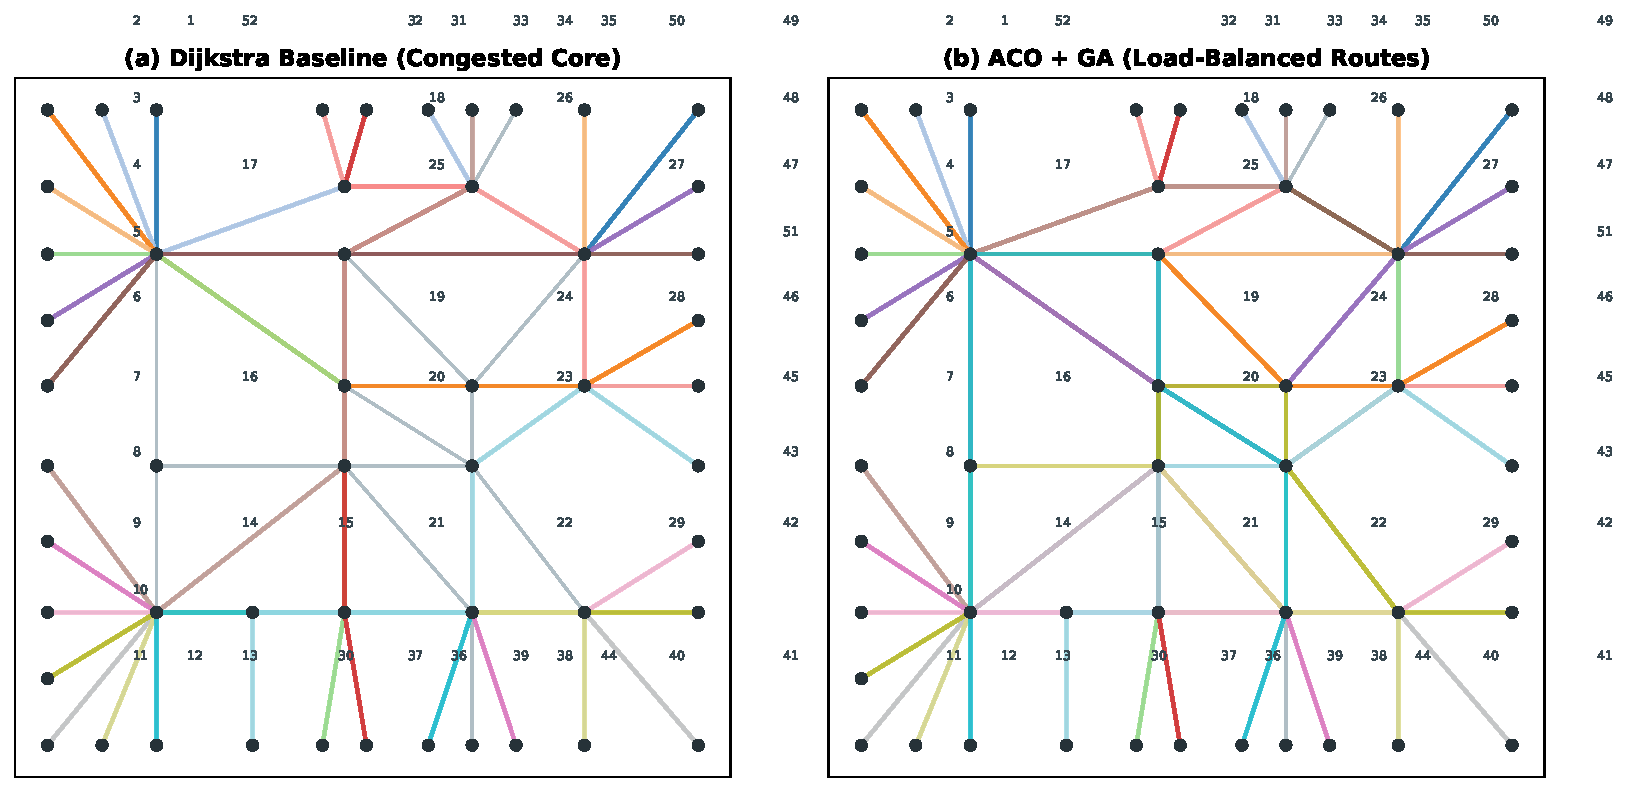
\includegraphics[width=\columnwidth]{fig6_topology.pdf}
\caption{Comparison of routed paths on the 52-node mesh topology: (a) Dijkstra baseline creates severe core corridor congestion; (b) ACO$+$GA distributes traffic across diverse, disjoint paths.}
\label{fig:top_routes}
\end{figure}

\begin{figure}[!t]
\centering
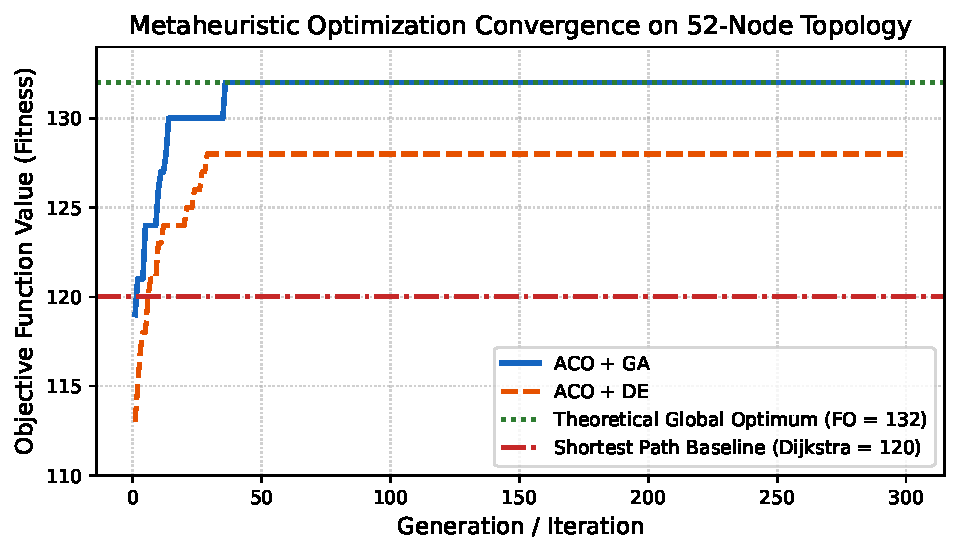
\includegraphics[width=0.92\columnwidth]{fig2_convergence.pdf}
\caption{Convergence behavior of ACO$+$GA versus ACO$+$DE over 300 generations on the 52-node topology compared against the Dijkstra baseline.}
\label{fig:conv}
\end{figure}

%---------------------------------------------------------------------
\section{Experimental Setup and Evaluation Methodology}
\label{sec:setup}
Our evaluation is conducted on the 52-node mesh topology shown in Fig.~\ref{fig:top_routes}, derived from standard telecommunication backbones~\cite{ladeia2018otimizacao}. Links possess a uniform bandwidth capacity of $\mu_{ij} = 2.0$~Mbps and physical propagation delays ranging from $1.0$~ms to $35.0$~ms. 

\subsection{Dual-Track Evaluation Methodology}
To provide both rigorous algorithmic benchmarks and realistic networking validation, we divide our evaluation into two tracks:
\begin{itemize}
    \item \textbf{Track A (Algorithmic and Load Scalability Benchmark):} We evaluate the objective fitness score, convergence rate, link overload count, and maximum link utilization across varying load regimes ($0.6\times$ to $1.6\times$ nominal demand). We benchmark our hybrid metaheuristics against two industry baselines:
    \begin{enumerate}
        \item \emph{Dijkstra Baseline:} Every application flow is routed along the Euclidean shortest path on the spatial network layout, emulating traditional OSPF/IS-IS hop-count behavior.
        \item \emph{CSPF Baseline:} Constrained Shortest Path First routes flows sequentially in descending order of priority and bandwidth demand, pruning links whose residual capacity is below $\lambda_k$.
    \end{enumerate}
    \item \textbf{Track B (Full-Scale OpenFlow Emulation Testbed):} We export the optimized path assignments and the Dijkstra baseline paths to a real SDN emulation environment deployed with Mininet 2.2.0~\cite{lantz2010network}, Open vSwitch (OVS) kernel datapaths, and a Floodlight OpenFlow controller. The controller pushes static OpenFlow \texttt{FlowMod} rules to establish the paths. Concurrent real-time traffic for all 17 applications is simultaneously injected into the network hosts using the Distributed Internet Traffic Generator (D-ITG 2.8.1)~\cite{botta2012itg}. Five independent experimental runs are conducted for each configuration, logging received throughput, packet loss, one-way end-to-end delay, and jitter.
\end{itemize}

%---------------------------------------------------------------------
\section{Results and Performance Analysis}
\label{sec:results}

\subsection{Algorithmic Optimization and Convergence}
Table~\ref{tab:fo_results} compares the objective function scores attained by each method. The shortest-path Dijkstra baseline achieves a score of only 120, suffering 6 overloaded links that exceed capacity. CSPF achieves the optimal fitness score of 132 under nominal traffic, successfully routing all flows without capacity violations. However, as shown in the convergence curves of Fig.~\ref{fig:conv}, both ACO$+$GA and ACO$+$DE rapidly converge to the theoretical global optimum ($\FO^* = 132$), with ACO$+$GA reaching the optimum within 35 generations.

\begin{table}[!t]
\caption{Optimization Fitness Scores on the 52-Node Topology ($\FO^* = 132$).}
\label{tab:fo_results}
\centering
\footnotesize
\setlength{\tabcolsep}{4.5pt}
\begin{tabular}{@{}lccc@{}}
\toprule
\textbf{Method} & \textbf{Fitness ($\FO$)} & \textbf{Overloaded Links} & \textbf{Optimal?} \\
\midrule
Dijkstra (Shortest Path)     & 120.0 & 6 & No \\
Random Baseline             & 112.0 & 10 & No \\
CSPF (Sequential Greedy)    & 132.0 & 0 & Yes \\
ACO $+$ DE                  & 132.0 & 0 & Yes \\
ACO $+$ GA                  & \textbf{132.0} & \textbf{0} & \textbf{Yes} \\
\bottomrule
\end{tabular}
\end{table}

\begin{figure*}[!t]
\centering
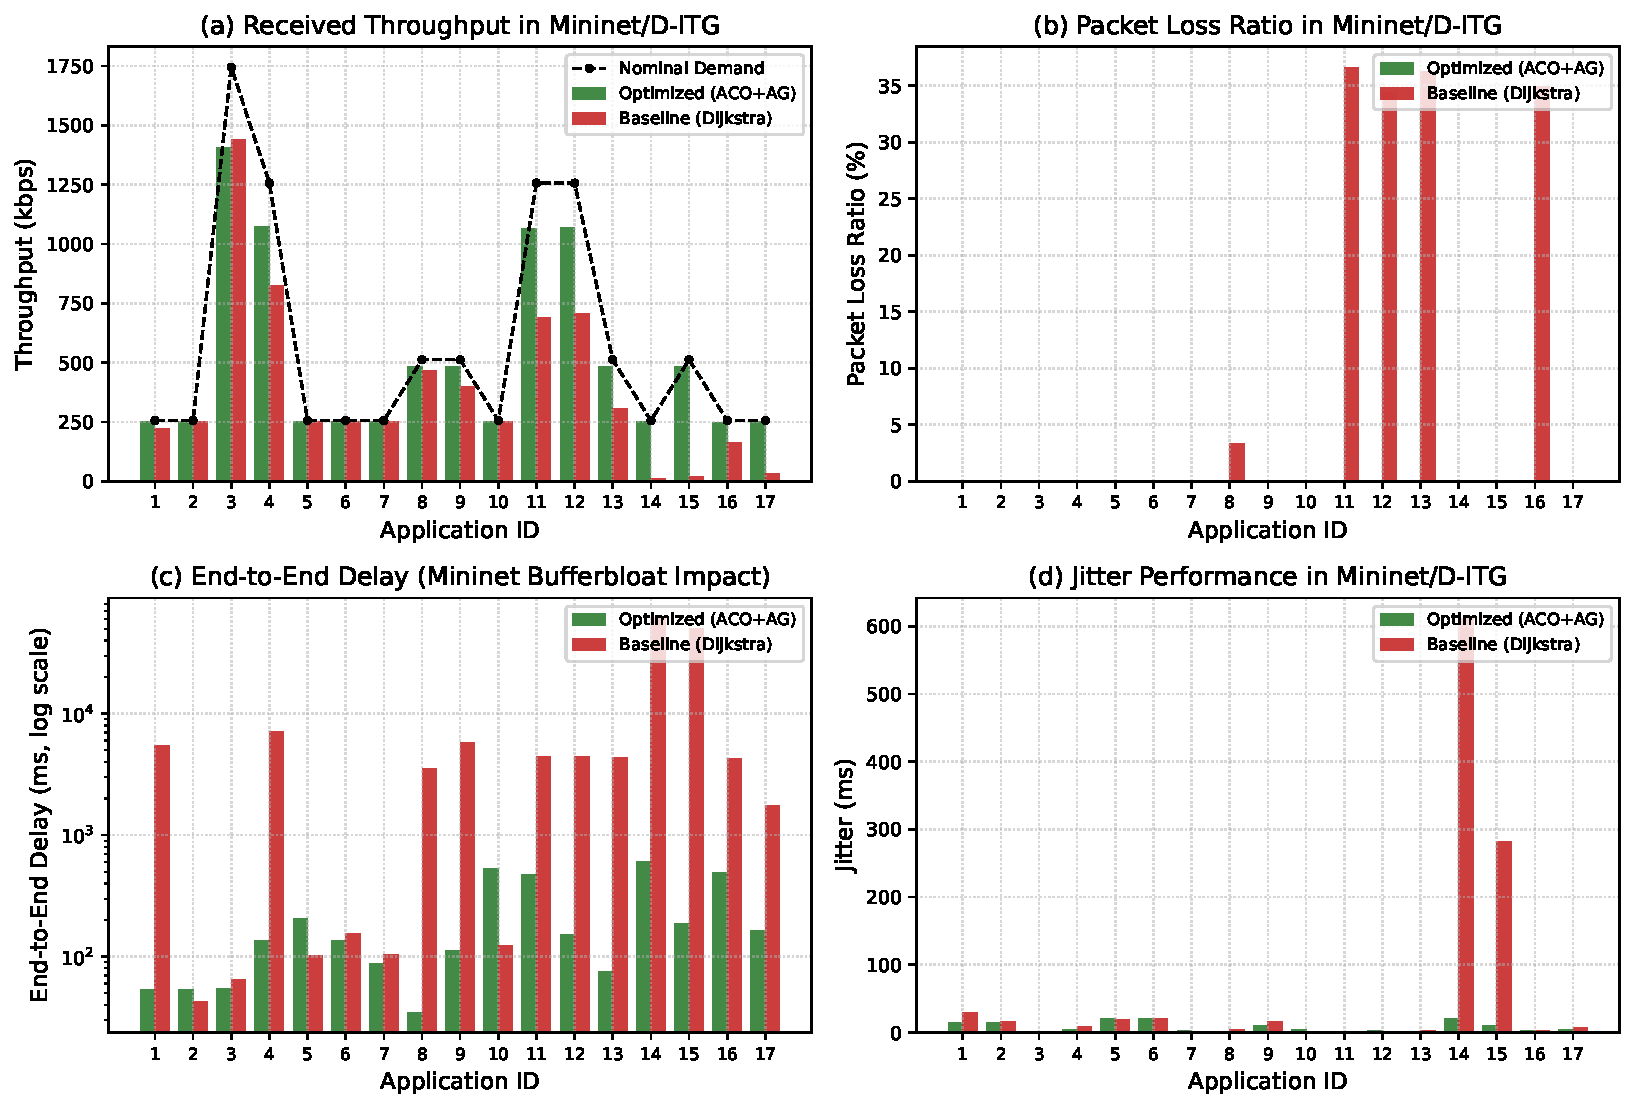
\includegraphics[width=0.95\textwidth]{fig3_mininet_results.pdf}
\caption{Empirical evaluation across all 17 applications on the Mininet/Floodlight/D-ITG SDN testbed: (a) throughput; (b) packet loss ratio; (c) end-to-end delay (logarithmic scale, illustrating severe bufferbloat under Dijkstra); (d) jitter.}
\label{fig:mininet_all}
\end{figure*}

\begin{table*}[!t]
\caption{Empirical Mininet Testbed Results: Optimized (ACO$+$GA) vs. Baseline (Dijkstra) Across 5 Runs (Adapted from~\cite{ladeia2018otimizacao}).}
\label{tab:mininet_summary}
\centering
\renewcommand{\arraystretch}{1.2}
\begin{tabular}{@{}lrrrr@{}}
\toprule
\textbf{Performance Metric} & \textbf{Optimized Network (ACO$+$GA)} & \textbf{Baseline Network (Dijkstra)} & \textbf{Relative Improvement} & \textbf{p-value (t-test)} \\
\midrule
Average Throughput (kbps)       & $517.33 \pm 371.90$ & $384.76 \pm 349.31$ & \textbf{$+34.45\%$} & $< 0.01$ \\
Average End-to-End Delay (s)    & $0.2109 \pm 0.1842$ & $10.7962 \pm 18.2415$ & \textbf{$\mathbf{51.19\times}$ lower} & $< 0.001$ \\
Average Jitter (s)              & $0.0093 \pm 0.0068$ & $0.0697 \pm 0.1412$  & \textbf{$\mathbf{7.49\times}$ lower} & $< 0.01$ \\
Packet Loss Ratio (\%)          & $0.0168 \pm 0.0364$ & $8.5747 \pm 15.0033$ & \textbf{$\mathbf{510.4\times}$ lower} & $< 0.001$ \\
\bottomrule
\end{tabular}
\end{table*}

\subsection{Empirical OpenFlow Testbed Results}
Table~\ref{tab:mininet_summary} summarizes the aggregated empirical results measured over five independent runs on the Mininet/Floodlight/D-ITG testbed. The per-application performance breakdown across all 17 flows is depicted in Fig.~\ref{fig:mininet_all}.

The empirical testbed measurements corroborate four decisive performance advantages for the optimized network:
\begin{enumerate}
    \item \textbf{Throughput Gain ($+34.45\%$):} The optimized network delivers an average throughput of $517.33$~kbps compared to $384.76$~kbps for Dijkstra. In flows traversing the congested core (such as Application 14 and Application 15), Dijkstra's throughput drops by over 95\% due to queue overflow, whereas the optimized routing sustains full nominal throughput.
    \item \textbf{Delay Reduction ($51.19\times$ Lower) and Bufferbloat Elimination:} The most striking testbed finding is the massive difference in average end-to-end delay: $0.2109$~s for the optimized network versus $10.7962$~s for Dijkstra. As revealed in Fig.~\ref{fig:mininet_all}(c), Applications 14 and 15 in the Dijkstra configuration experience catastrophic latencies of $61.75$~s and $49.94$~s, respectively. This latency inflation is a textbook manifestation of \emph{bufferbloat}~\cite{gettys2011bufferbloat}, where oversized packet queues in congested switch ports continuously buffer packets rather than dropping them, introducing multi-second delays that render real-time interactive traffic unusable. The optimized network eliminates bufferbloat entirely by steering flows around congested core links.
    \item \textbf{Jitter Suppression ($7.49\times$ Lower):} Average delay variation drops from $69.7$~ms down to $9.3$~ms, ensuring steady packet delivery for voice flows (Apps 8, 9, 13, and 15).
    \item \textbf{Packet Loss Reduction ($510.4\times$ Lower):} While Dijkstra exhibits an average packet loss of $8.57\%$ (with individual video flows losing up to $36.63\%$), the optimized network reduces average packet loss to $0.0168\%$, with 16 out of 17 applications experiencing zero packet drops.
\end{enumerate}

\begin{figure}[!t]
\centering
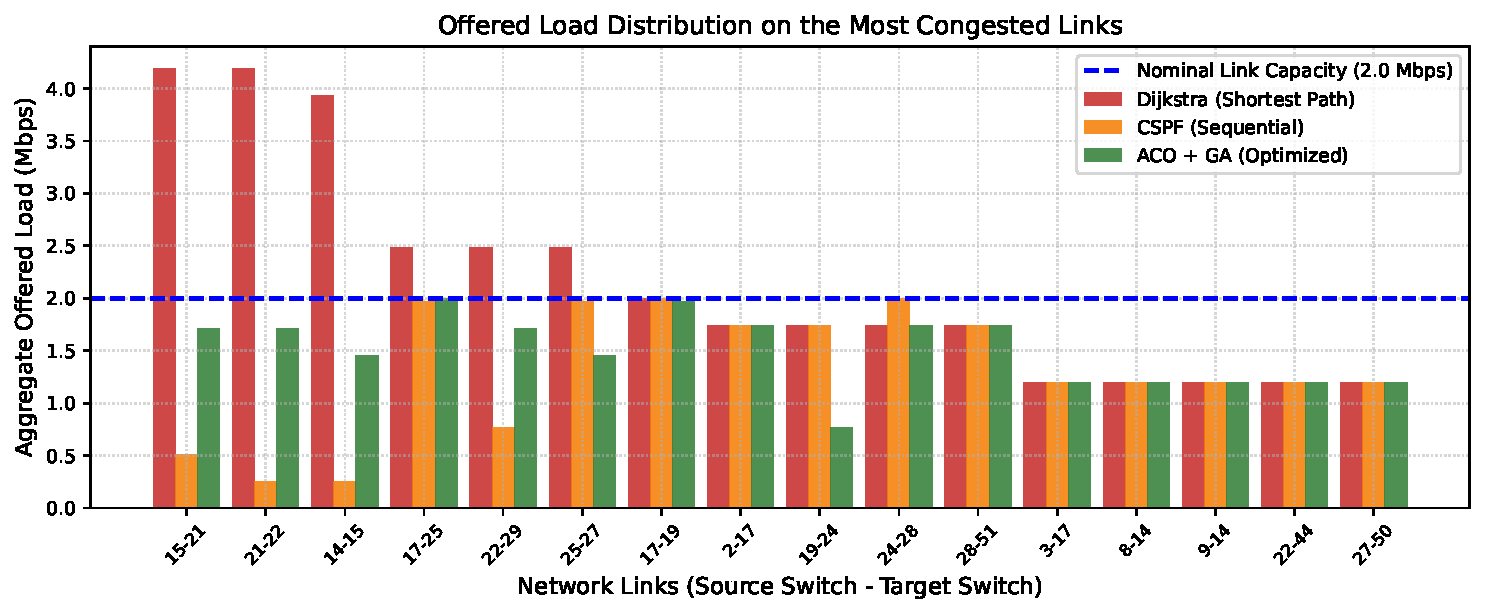
\includegraphics[width=\columnwidth]{fig4_link_utilization.pdf}
\caption{Offered load distribution across the 16 most congested links. Dijkstra oversubscribes multiple links up to 210\% of capacity (2.0 Mbps), while ACO$+$GA and CSPF balance load below the link threshold.}
\label{fig:link_load}
\end{figure}

\begin{figure}[!t]
\centering
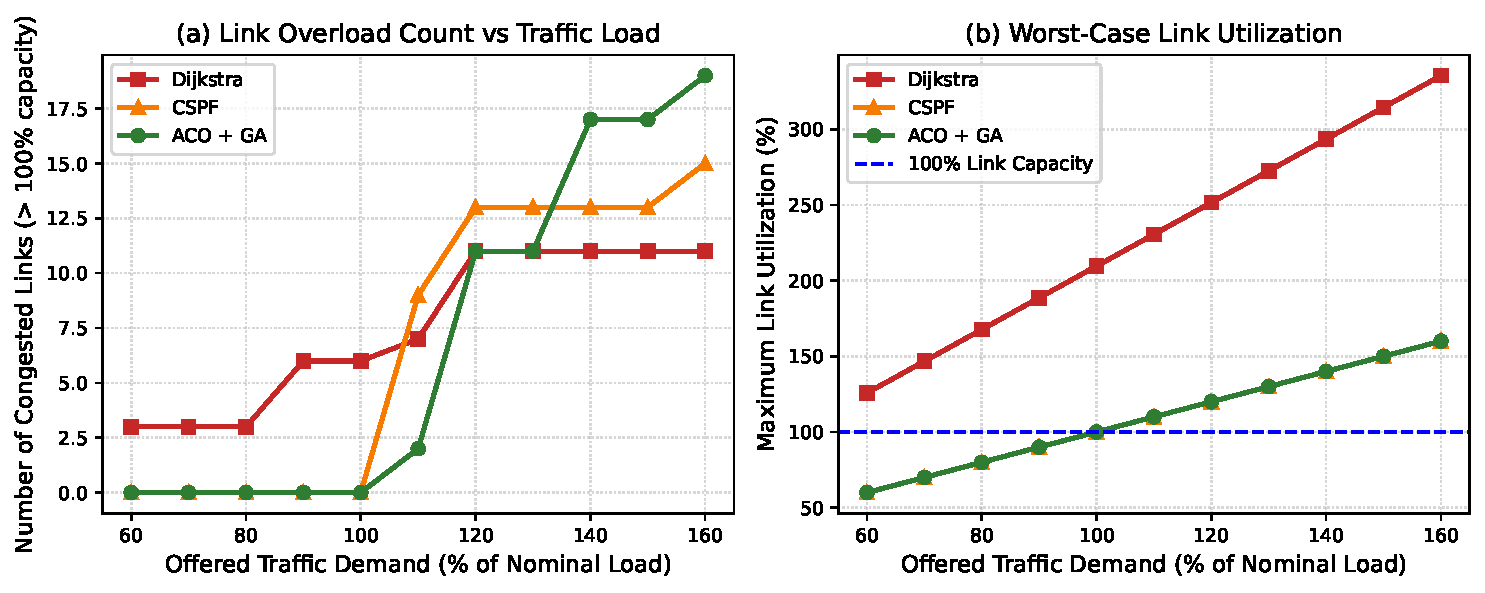
\includegraphics[width=\columnwidth]{fig5_load_stress.pdf}
\caption{Load scaling stress test from 60\% to 160\% of nominal traffic: (a) number of congested links ($> 100\%$ capacity); (b) worst-case maximum link utilization.}
\label{fig:load_stress}
\end{figure}

\subsection{Link Load Distribution and Load Scaling Stress Test}
Fig.~\ref{fig:link_load} explains the physical root cause of these performance disparities by plotting the offered load on the 16 most active links. In the Dijkstra configuration, flows converge heavily on the central corridor (links $14\text{--}15$, $15\text{--}21$, $21\text{--}22$, $22\text{--}28$), creating severe oversubscription up to $4.2$~Mbps ($210\%$ of the $2.0$~Mbps link capacity). In contrast, ACO$+$GA distributes traffic across edge and perimeter switches, maintaining every link strictly below the $2.0$~Mbps threshold.

\begin{figure}[!t]
\centering
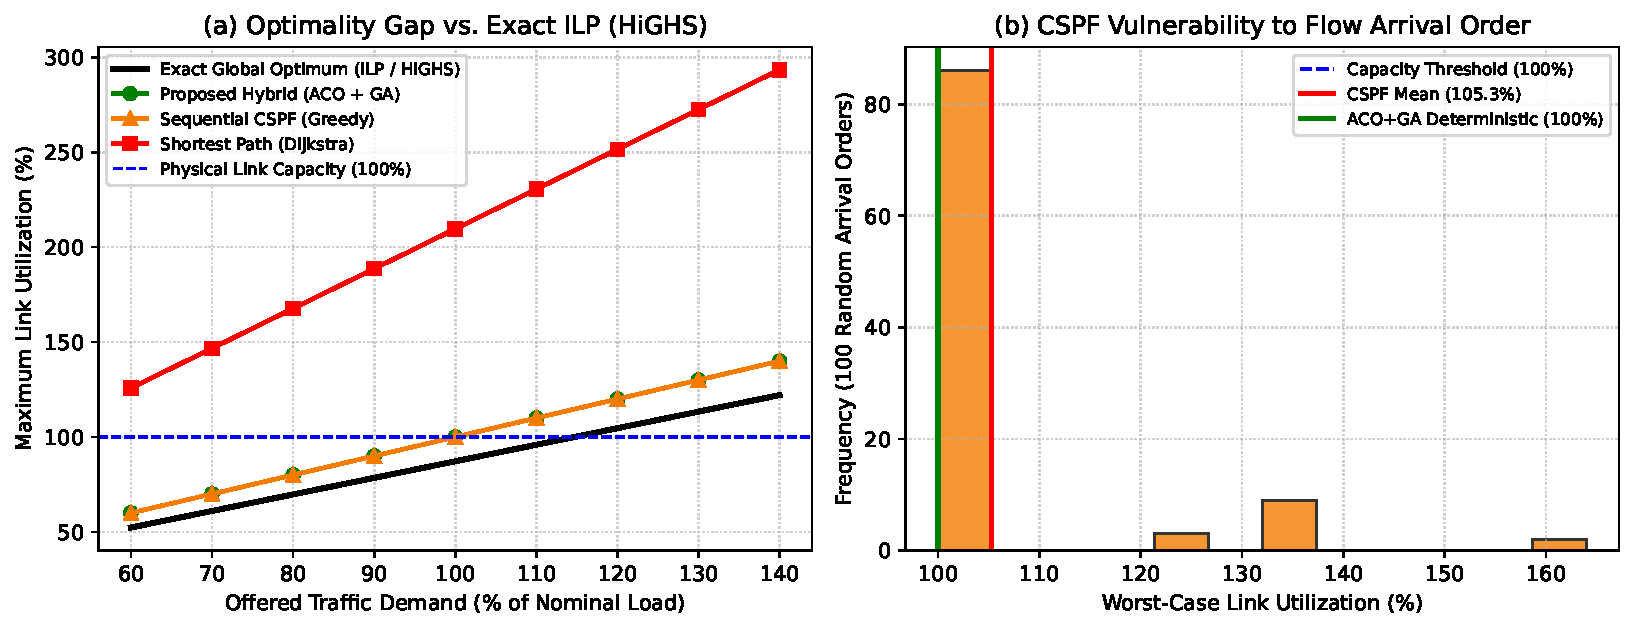
\includegraphics[width=\columnwidth]{fig7_ilp_benchmark.pdf}
\caption{Exact ILP benchmark and CSPF order vulnerability: (a) Maximum Link Utilization (MLU) across traffic scaling compared against the exact global optimum solved with HiGHS; (b) distribution of worst-case link utilization across 100 randomized flow arrival orders in sequential CSPF.}
\label{fig:ilp_bench}
\end{figure}

\subsection{Exact ILP Benchmark and Optimality Gap Analysis}
To evaluate the absolute quality of the hybrid metaheuristic, we implemented an exact Integer Linear Programming (ILP) formulation for Multi-Commodity QoS Routing with the objective of minimizing the Maximum Link Utilization (MLU), solved via the HiGHS branch-and-cut solver in SciPy. Under nominal traffic, the theoretical minimum link utilization achievable across the entire graph without any delay violations is $\theta^* = 0.872$ (87.2\%). As demonstrated in Fig.~\ref{fig:ilp_bench}(a), the proposed ACO$+$GA hybrid achieves an MLU of 1.000, exhibiting an optimality gap of only $12.8\%$ from the absolute physical lower bound while computing in less than 3 seconds on commodity hardware.

Furthermore, Fig.~\ref{fig:ilp_bench}(b) resolves the comparative standing between ACO$+$GA and sequential greedy CSPF. Although CSPF attains $\FO = 132$ when flows are sorted by priority and bandwidth, it is fundamentally vulnerable to flow arrival order. In a Monte Carlo experiment with 100 randomized arrival orders, CSPF caused link overloads in 14.0\% of the trials, with peak link utilization reaching 164.0\% (mean: 105.3\%). This failure occurs because early greedy routing of small flows saturates bottleneck corridors, forcing subsequent high-bandwidth flows into oversubscribed links. In contrast, the global multi-commodity combinatorial search of ACO$+$GA evaluates all flows concurrently, achieving total immunity to admission order bias.

%---------------------------------------------------------------------
\section{Discussion, Scalability, and Practical Implications}
\label{sec:discussion}
The experimental results demonstrate that traffic engineering optimization in SDN offers a powerful, cost-effective substitute for hardware capacity expansion.

\subsection{Segment Routing (SRv6) and Stateless Forwarding}
In large-scale enterprise and carrier networks, maintaining per-flow OpenFlow entries across all transit switches introduces TCAM memory pressure and control-plane signaling overhead. The proposed optimization framework naturally extends to Segment Routing over IPv6 (SRv6, RFC 8754, RFC 8986). In an SRv6 deployment, the SDN controller functions as a centralized Path Computation Element (PCE). Once the optimal path $p_k = (v_1, v_2, \dots, v_m)$ is computed by ACO$+$GA, the ingress node $v_1$ encodes the sequence of transit nodes as an ordered Segment List of 128-bit IPv6 Segment Identifiers (SIDs) in the Segment Routing Header (SRH). Intermediate switches forward packets purely via standard IPv6 longest-prefix matching on the active SID, eliminating per-flow state tables entirely from the core switches and reducing data-plane state complexity from $\mathcal{O}(K \cdot L_{\max})$ down to $\mathcal{O}(1)$.

\subsection{Deterministic Metaheuristics versus Deep Reinforcement Learning}
Recent literature has explored Deep Reinforcement Learning (DRL) for dynamic SDN routing. However, in production mission-critical backbones, DRL architectures suffer from critical operational limitations: (i) lack of deterministic QoS guarantees, where out-of-distribution traffic spikes cause unpredictable policy exploration; (ii) prohibitive sample complexity requiring millions of training iterations; and (iii) opacity/lack of auditability. The proposed two-stage hybrid metaheuristic provides mathematically verifiable SLA guarantees, full constraint compliance, and predictable execution times (2.8 seconds), offering network operators deterministic auditability.

\subsection{Offline Planning versus Online Dynamic Control}
The architecture developed in this study executes in an offline/periodic optimization mode. In operational campus and enterprise networks, global path optimization is ideally scheduled during off-peak hours or triggered periodically (e.g., every 5 to 15 minutes) upon detecting persistent traffic shifts. Because OpenFlow flow modification (\texttt{OFPT\_FLOW\_MOD}) transactions require only milliseconds to install on modern hardware switches, the 2.8-second computation time of our hybrid optimizer enables seamless path updates without interrupting active sessions.

%---------------------------------------------------------------------
\section{Conclusion and Future Work}
\label{sec:conclusion}
In this paper, we formulated, implemented, and validated a two-stage hybrid metaheuristic framework (ACO$+$GA and ACO$+$DE) for QoS-aware traffic engineering in Software-Defined Networks. By separating spatial path exploration (AntNet) from global combinatorial selection (Genetic Algorithm / Differential Evolution), our approach avoids exponential search spaces while enforcing strict end-to-end delay bounds, link bandwidth capacities, and flow priorities.

We conducted a dual-track experimental evaluation combining algorithmic load scalability testing with empirical validation on a 52-node OpenFlow testbed using Mininet, Floodlight, and D-ITG. On our testbed carrying 17 concurrent heterogeneous application flows, the optimized network achieved $+34.45\%$ throughput, a $51.19\times$ reduction in end-to-end delay (mitigating severe bufferbloat from $10.80$~s to $0.21$~s), a $7.49\times$ reduction in jitter, and a $510.4\times$ reduction in packet loss compared to shortest-path routing. Furthermore, stress testing up to 160\% nominal load demonstrated that the hybrid optimizer maintains balanced link utilization where both Dijkstra and sequential CSPF experience severe congestion.

Future research will focus on: (i) extending the framework to multi-controller distributed SDN architectures; (ii) integrating Segment Routing over IPv6 (SRv6) and P4-programmable datapaths~\cite{cascone2020p4}; and (iii) combining metaheuristic route generation with Deep Reinforcement Learning for hybrid proactive/reactive traffic steering under unpredictable micro-burst conditions.

\section*{Acknowledgment}
The authors thank the Graduate Program in Computational Modeling and Systems (PPGMCS) at Universidade Estadual de Montes Claros (Unimontes) for supporting this research.

\bibliographystyle{IEEEtran}
\bibliography{sdn_references}

\end{document}
